% !TEX root=../main.tex
\documentclass[beamer]{standalone}
\begin{document}

% Differentiable rendering
\begin{frame}{Related-work}
\framesubtitle{Gradient Filtering}

\begin{itemize}
    \item "Laplacian Smooth Gradient Descent", Osher et al, 2019 ICLR
    \begin{figure}[h]
        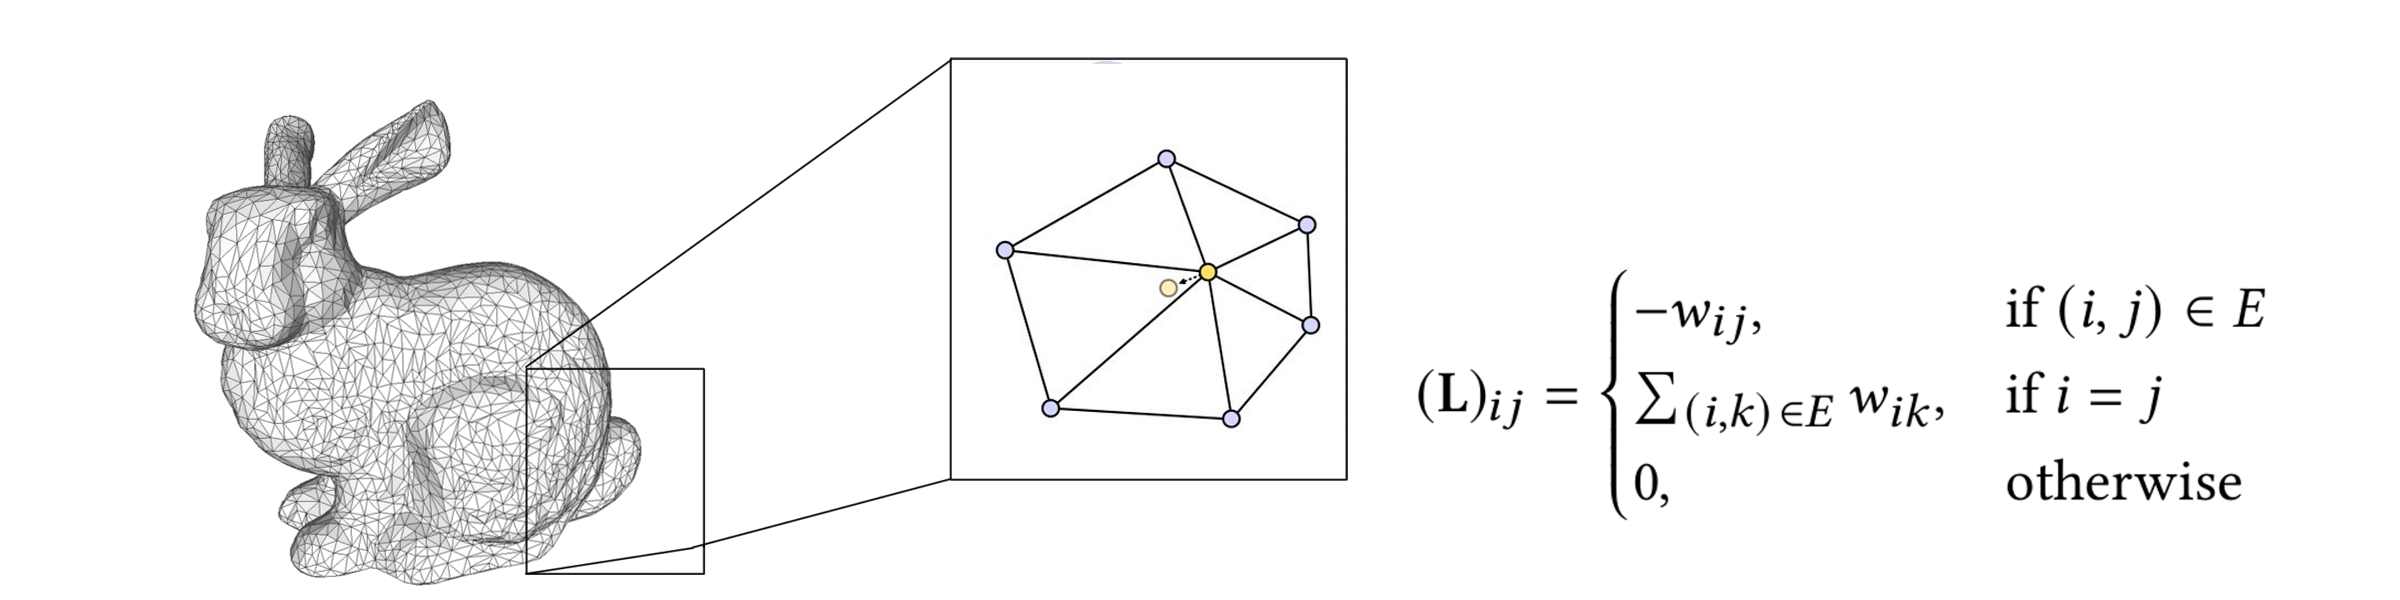
\includegraphics[width=0.8\linewidth]{./figures/related-work-1.png}
    \end{figure}
    \begin{enumerate}
        \item machine learning paper 
        \item smoothing method for stochastic gradient descent method (SGD) or GD
        \item multiplying the usual (stochastic) gradient by a one-dimensional discrete Laplacian
    \end{enumerate}

\end{itemize}

\note[item] {

    }
\end{frame}

% Mesh propertices / laplace
\begin{frame}{Related-work}
\framesubtitle{Gradient Filtering}
\begin{itemize}
    \item "Large steps in the Inverse Rendering", \\ 
    Baptiste Nicolet, Alec Jacobson and Wenzel Jackob, 2021 SIGGRAPH ASIA
    \begin{figure}[h]
        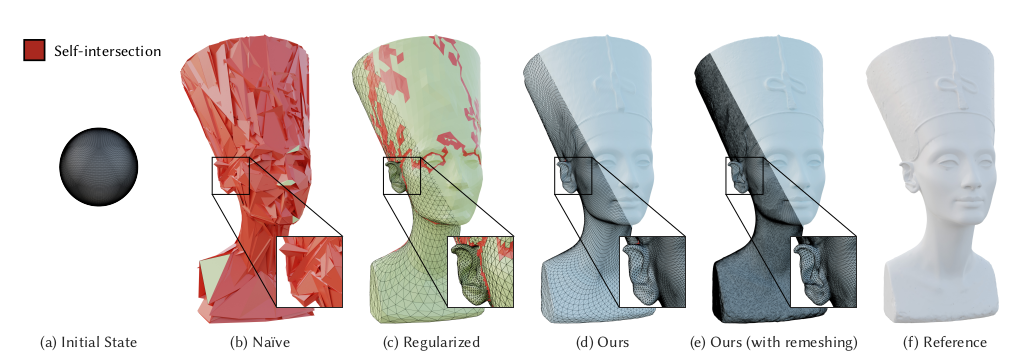
\includegraphics[width=0.8\linewidth]{./figures/related-work-2.png}
    \end{figure}
    \begin{enumerate}
        \item Quasi-Newton's method for gradient descent using the mesh properties
        \item Main idea: gradient filtering with the properties of paramters
    \end{enumerate}
\end{itemize}
    
% notes %
\note[item]{
    }   
\end{frame}
\end{document}
